% PROTOKOLL Action Item
\documentclass[
   draft=false
  ,paper=a4
  ,twoside=false
  ,fontsize=11pt
  ,headsepline
  ,DIV=11
  ,parskip=full+
  ,titlepage
]{scrartcl} % copied from Thesis Template from HAW

\usepackage[ngerman,english]{babel}

\usepackage[T1]{fontenc}
\usepackage[utf8]{inputenc}

\usepackage[
    left  =4em
   ,right =4em
   ,top   =5em
   ,bottom=5em
]{geometry}

\usepackage{longtable}
\usepackage[german,refpage]{nomencl}

\usepackage{float}
%\usepackage{enumitem}
\usepackage{paralist} %compactitem
\usepackage{graphicx}
%\usepackage{url}



\usepackage{hyperref} % for a better experience

\hypersetup{
   colorlinks=true % if false - links get colored frames
  ,linkcolor=black % color of tex intern links
  ,urlcolor=blue   % color of url links
  ,citecolor=black
}

\usepackage{amsmath}

\usepackage{array}   % for \newcolumntype macro
\newcolumntype{L}{>{$}l<{$}} % math-mode version of "l" column type
\newcolumntype{R}{>{$}r<{$}} % math-mode version of "r" column type
\newcolumntype{C}{>{$}c<{$}} % math-mode version of "c" column type

\usepackage{color}
\definecolor{black}{rgb}{0,0,0}
\definecolor{darkgray}{rgb}{0.2,0.2,0.2}
\definecolor{lightgray}{rgb}{0.9,0.9,0.9}
\definecolor{blue}{rgb}{0.0,0.0,0.9}
\definecolor{orange}{rgb}{0.7,0.3,0.0}
\definecolor{green}{rgb}{0.0,0.7,0.0}
\definecolor{red}{rgb}{0.9,0.0,0.0}

\usepackage{listings, lstautogobble}
\lstset{%
   language=bash
  ,frame=single
  ,numbers=left
  ,numberstyle=\tiny\color{darkgray}
  ,stepnumber=1
  ,numbersep=5pt
  ,backgroundcolor=\color{lightgray}
  ,showspaces=false
  ,keepspaces=true
  ,autogobble=true 
  ,breaklines=true
  ,tabsize=2
  , 
  ,basicstyle=\footnotesize\ttfamily\color{black}
  ,identifierstyle=\color{black}
  ,keywordstyle=[1]\color{blue}\textbf
  ,keywordstyle=[2]\color{red}\textbf
  ,stringstyle=\color{green}
  ,commentstyle=\color{darkgray}\textit
}
  
\usepackage{caption}
\usepackage{colortbl}
\definecolor{tabgrey}{rgb}{0.85,0.85,0.85}
%using minted because of the hashtag in bash

\sloppy
\clubpenalty=10000
\widowpenalty=10000
\displaywidowpenalty=10000


\usepackage{filecontents}

\usepackage{natbib}



% set font 
%\renewcommand{\familydefault}{\sfdefault}
\usepackage{times}

\begin{document}

\selectlanguage{ngerman}
% ----------------------------------------------------------------------------
% ---------------------------------------------------------- HIER WAS MACHEN -
% -------------------------------- Metadaten wie namen und Gruppentreffen etc-
\title{The git must flow}
\subtitle{a git survival kit - german version}
\author{kafawi}
\date{\today}

\publishers{%
	\normalfont\normalsize%
	\parbox{0.8\linewidth}{\centering
	  Dieses Dokument ist speziell für das Praktikum des ESE 
	  Moduls 2017 des Studienganges Technische Informatik der HAW Hamburg
	  erstellt worden und dient der Zusamenarbeit der Gruppe LANKE. 
		Es werden hier die Grundideen mit dem Umgang mit git und
		dem \"{}flow\"{} erklärt. Die Commit Message Struktur sowie die 
		Branchstruktur wird hier beschlossen. 
	}
}

\maketitle
\setcounter{page}{1}
\tableofcontents
\flushleft


\section{Einleitung}

  Dies soll ein Crashkurs in Sachen Git für dieses Projekt darstellen.
  Es wird sich hier auf das Nötigste beschränkt. Für tiefergreifende
  Informationen sollten externe Quellen verwendet werden, wie
  \citep{ProGit}, welches online frei zur verfügung steht.
  \newline
  
  \begin{minipage}[t]{0.45\linewidth}
	Der Quellcode in den Listings zeigt nur die Gitbefehle, wie sie in 
	einem Terminal verwendet werden. Die Ausgaben werden nicht aufgeführt.
	Als Prompt wird $\$ $ verwendet. Davor steht der aktuelle Branch
	(checktout branch) in Klammern $(branchname)\$$. Kommentare werden mit
	einem Voranngeführten $\# $ eingeleitet. 
  \end{minipage}%
  \hfill
  \begin{minipage}[t]{0.5\linewidth}
    \begin{lstlisting}
      (master)$ git checkout develop
      # Update develop
      (develop)$ git pull
      (develop)$ git checkout -b feature/myfeature
      (feature/myfeature)$ ...
    \end{lstlisting}
  \end{minipage}%
  
  Zunächst wird der Workflow, welcher in diesem Projekt 
  praktiziert werden soll, erklärt. Darauf folgen die Konventionen
  im Umgag mit Git, wie die Struktur der Commit Messages. Darauf 
  Folgt eine Auffrischung der Git Befehle. Im Letzten Kapitel werden
  nützliche Tricks und Kniffe vorgestellt.
	  
\newpage

\section{Workflow}
  Wegen der sehr kleinen Anzahl von Entwicklern, wird ein 
  zentralisierter Workflow angewendet, d.h. wir haben ein 
  Referenzrepro auf einem Server, welcher uns den aktuellen
  Stand für unsere lokalen Repros anbietet. Dabei haben wir 
  zwei Hauptbranches und mehrere dynamische Featurebranches, 
  auf denen hauptsächlich Entwickelt wird. Dargestellt ist dies
  in der Abbildung \ref{fig:workflow}. 
    
\begin{figure}[H]
  	\centering
    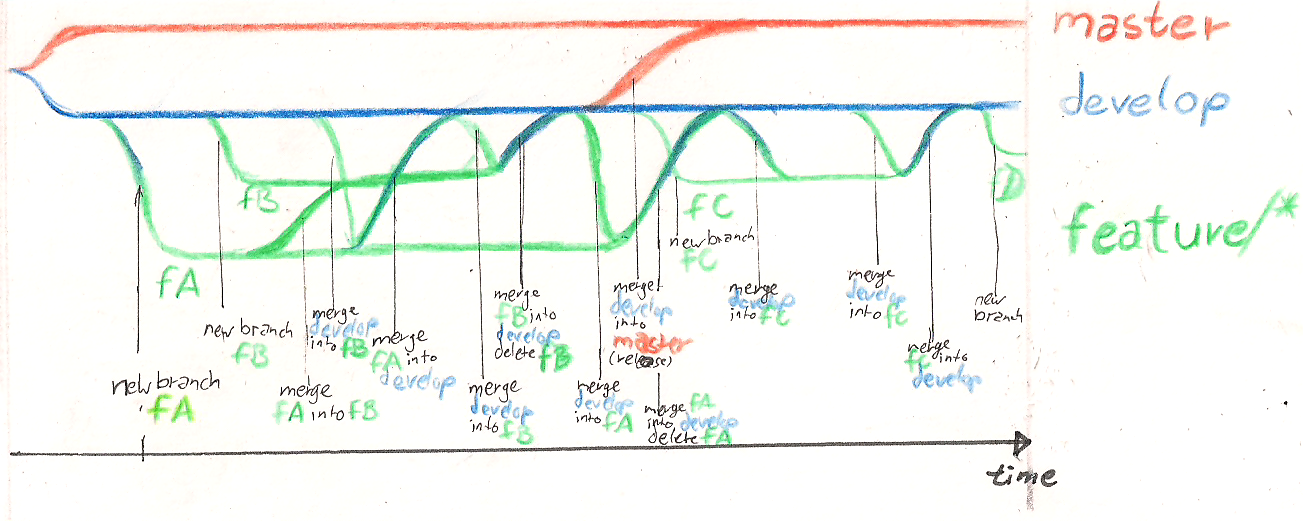
\includegraphics[width=0.8\textwidth]{./IMG/gitworkflow.png}
    \caption[workflow]{%
    Der Workflow, wie er in diesem Projekt 
    stattfinden soll, ist hier dargestellt. Der Masterbranch 
    \texttt{master} ist für die Releases bestimmt und nur der 
    \texttt{develop} wird kurz vor einem Release gemerged. 
    Vom Entwicklungsbranch
    \texttt{develop} werden die jeweiligen Featurebanches 
    \texttt{feature/*} abgeleitet und auf diesen wird in kleinen Teams 
    gearbeitet. Wenn ein Feature fertig gestellt wird, wird dieses auf dem
    mit dem \texttt{remote} upgedateten \texttt{develop} eingepflegt.
    Wird der Featurebranch nicht mehr gebraucht, wird dieser 
    lokal und im remote gelöscht (\texttt{git branch -dr origin/feature/*}).
    }%
    \label{fig:workflow}
\end{figure}

  
  \begin{description}
    \item[master] Dieser \texttt{branch} ist nur für Realeses bestimmt, 
    und wird nur mit dem \texttt{develop} gemerged. 
    (neuster Stand des Projektes für den nächsten Praktikumstermine)
    \item[develop] Stellt die Basis für jedes \texttt{feature/*} da. Jedes
    einzelne \texttt{feature/*} kann in den \texttt{develop} gemerged werden,
    sobald dieser für annehmbar (qualitativer Inhalt) befunden wurde.     
    \item[feature/*] Hier werden die einzelnen Tasks in Code umgewandelt.
    Diese \texttt{branches} leiten sich von den
    dem \texttt{develop} ab und werde in diesen bei der Fertigstellung des
    \texttt{feature/*} zurückgeführt und ggf. gelöscht. Es kann zwischen
    den \texttt{feature/*} auch gemerged werden, falls diese 
    ein bestimmtes \texttt{feature/fA} dringend braucht, welches sich 
    noch nicht auf dem develop befindet, da es z.B. in der Review befindet.
    Vor jedem merge in den \texttt{develop} muss das \texttt{feature/myF}
    den aktuellen Stand des \texttt{origin/develop} in sich integrieren
    (mergen). 
  \end{description}
  
  
  \subsection{Zusammenarbeit im Workflow}
    Wenn mehrere Entwickler an einem \texttt{feature/*} arbeiten, dann
    müssen sie sich miteinander Absprechen, bzw. vor jedem Sprint, wird 
    der aktuelle Stand dieses \texttt{origin/feature/*} auf den lokalen
    \texttt{branches} angeglichen. 
    
  \subsubsection{Erstellung eines features und veröffentlichen}
    
    
  \begin{minipage}[t]{0.25\linewidth}
	  Im nebenstehen Listing wird ein Ablauf
    beschrieben, wie man ein neuen Featurebranch anlegt und 
    diesen veröffentlicht.
    Dabei kann es auch vorkommen, dass ein anderer Entwickler einen
    Featurebranch mit gleicher Intention angelegt hat und diesen vorher 
    schon veröffentlicht hat. Dann muss man seinen eigenen Branch
    mit dem schon vorhandenen zusammenführen.
    Wichtig ist, dass jeder \texttt{feature/*} von einem aktuellen 
    \texttt{develop} abstammt. 
  \end{minipage}% 
  \hfill
  \begin{minipage}[t]{0.65\linewidth}
    \begin{lstlisting}
      (master)$ git checkout develop
      # Update develop
      (develop)$ git pull
      # create and checkout new branch
      (develop)$ git checkout -b feature/fA
      # working some on some files and stage them
      (feature/fA)$ ...
      (feature/fA)$ git commit
      # looking for new branches in remote
      (feature/fA)$ git fetch
      (feature/fA)$ git branch -a
      # two possibilities
      #     1. my feature is not a existing topic
      #        -> publish
      (feature/fA)$ git push -u origin feature/fA
      #     2. my partner already has a fAA-branch
      (feature/fA)$ git checkout --track origin/feature/fAA
      (feature/fAA)$ git merge feature/fA
      # delete my branch
      (feature/fAA)$ git branch -d feature/fA
      (feature/fAA)$ git push
    \end{lstlisting}
  \end{minipage}%
    
  \subsubsection{Arbeiten an einem öffentlichen Feature}
  
  \begin{minipage}[t]{0.25\linewidth}
     Es wird zunächst der featurebranch lokal auf den neusten Stand gebracht.
     Dann sollte man erstmal angucken, was sich in geändert hat.
     Nach getaner Arbeit wird \texttt{feature/*} aktualisiert und 
     und entsprechend getestet. Erst dann wird \texttt{feature/*} auf 
     das remote gepusht.
  \end{minipage}%
  \hfill
  \begin{minipage}[t]{0.65\linewidth}
    \begin{lstlisting}
      # update develop
      (develop)$ git pull
      # get featurebranch fA 
      # if not existing
          (develop)$ git checkout --track origin/feature/fA
      # else
          (develop)$ git checkout feature/fA
          (feature/fA)$ git pull
      # whats new?
      (feature/fA)$ git log --since=1.weeks
      # starting with Sprint and commit
      (feature/fA)$ ...
      (feature/fA)$ git commit
      # update from repro
      (feature/fA)$ git fetch
      # while a new version of fA is online
          (feature/fA)$ git merge origin/feature/fA
          # testing after merge 
          (feature/fA)$ ...
          (feature/fA)$ git commit
          (feature/fA)$ git fetch 
      # publish / push
      (feature/fA)$ git push 
    \end{lstlisting}
  \end{minipage}%
  
  
  \subsubsection{Feature in den develop mergen}
  \begin{minipage}[t]{0.25\linewidth}
	  Das Feature ist aktuell und fertig geprüft, sodass es 
	  in den \texttt{develop} überführt werden kann. 
	  So wird zunächst der lokale \texttt{develop} geupdatet und
	  anschließend in den \texttt{feature/*} eingefügt. Dann 
	  werden Tests durchgeführt, ggf. Konflikte gelöst und anschließend
	  wird der \texttt{feature/*} in den \texttt{develop} einpflegt.
	  Wenn \texttt{feature/*} nicht mehr gebraucht wird, so wird dieser
	  vom lokalen und remote gelöscht.
  \end{minipage}%
  \hfill
  \begin{minipage}[t]{0.65\linewidth}
    \begin{lstlisting}
      (feature/fA)$ git checkout develop
      # Update develop
      (develop)$ git pull
      # do : 
          #switch to feature 
          (develop)$ git checkout feature/fA 
          # merge devolop into feature
          (feature/fA)$ git merge develop
          # testing
          (feature/fA)$ ...
          (feature/fA)$ git commit
          (feature/fA)$ git checkout develop
          # update develop again
          (develop)$ pull
      # while ( develop changes) -> do 
      (develop)$ git merge feature/fA
      # if feature is no longer needed
          # delete lokal
          (develop)$ git branch -d feature/fA 
          # delete remote  
          (develop)$ git push origin :feature/fA
          (develop)$ git branch -dr origin/feature/fA
    \end{lstlisting}
  \end{minipage}%
  
  \subsubsection{Realese}
  
  \begin{minipage}[t]{0.25\linewidth}
     Zu einer gewissen Zeit wird dem \texttt{master} der \texttt{develop}
     einverleibt. Dabei sollte sich auf \texttt{develop} ein vorzeigbarer
     Snapshot des Projektes befinden. Gegebenen falls kann man hier 
     dem Commit einen Tag geben. 
     Es wird aber ein kommentierter Tag bevorzugt.
  \end{minipage}%
  \hfill
  \begin{minipage}[t]{0.65\linewidth}
    \begin{lstlisting}
      # update develop
      (develop)$ git pull
      # update master
      (develop)$ git checkout master
      (master)$ git pull
      # merge develop into master
      (master)$ git merge develop
      # publish
      (master)$ git push
      # tagging
      (master)$ git tag -a v0.1
      (master)$ git push origin v0.1
    \end{lstlisting}
  \end{minipage}%
  
\newpage
  
\section{Konventionen}
  An diese Regeln sollte sich jeder Entwickler halten. Diese Regeln
  sorgen dafür, dass sich der Workflow einstellen kann und es zu keinen
  komischen Ausfällen kommt.
\begin{itemize}
	\item update before you work (update = pull = fetch + merge)
	\item update before you merge and push
	\item never rebase in an public branch
	\item never use git commit --amend to a published commit
	\item write commit messages in an editor with a template 
	\item all feature branches start with \texttt{feature/}
\end{itemize}
	\newpage
\subsection{Git Commit Message}
  Es wird die Grundstrukur der AngularJS Communitiy \citep{AngularJS}
  verwendet und auf unsere Bedürfnisse angepasst. 
  Die Commit messages werden in Englisch verfasst.
  
  \subsubsection{Struktur / template}
    \begin{minipage}[t]{0.45\linewidth}
      Ein Template ist in der Datei \texttt{.gitmessage} im Wurzelverzeichnis 
      unseres Projektes und wird mit 
      \newline 
      \scriptsize 
      \texttt{git config commit.template $"$.gitmessage$"$}
      \newline
    \normalsize
  eingepflegt. Diese Vorlage wird in deinen Editor geladen,
   wenn ein Commit ohne $"$-m$"$ Flag aufgerufen wird. 
  \end{minipage}%
  \hfill
  \begin{minipage}[t]{0.45\linewidth}
    \begin{lstlisting}
      <type>(<scope>): <subject>
      BLANKLINE
      <body>
      BLANKLINE
      <footer>
      --- EXAMPLE ---
      docs(RDD): Add stakeholder list
      
      Stakeholder are a hint, how we have to 
      designe our Project and how we have to 
      behave.
      
      Close stakeholder card
    \end{lstlisting}
  \end{minipage}%
  \newline
  \begin{compactitem}
    \item[head:]  Hier werden die wichtigesten Informationen zusammengefasst
    \begin{compactitem}
               \item  Er darf maximal 50 Zeichen lang sein
    \end{compactitem}
   
      \begin{compactitem}
         \item[<type>:] Typ des Commits, welche da sind:
            \begin{compactitem}
               \item[docs:]  Änderungen in der Documentation
               \item[feat:]  generell Änderung am Produktcode
               \item[test:]  Tests: keine Änderung am Produktcode
               \item[refac:] Refactoring am Produktcode
               \item[fix:]   gefixte Bugs
               \item[style:] änderung am Style (Einrückung etc.)
            \end{compactitem}
         \item[<scope>:] optional
            \begin{compactitem}
              \item Datei, Module, Layer auf die sich die Änderung
                 bezeiht       
              \item Wenn mehrere betroffen sind: (*) und Liste im <body>
            \end{compactitem} 
              
         \item[<subject>:] Was bewirkt die Änderung im Kern?
            \begin{compactitem}
              \item $"$ If applied, this commit will <subject> $"$
              \item Imparativ und Präsens       
              \item Beginnend mit einem Großbuchstaben
              \item Endet ohne Punkt
            \end{compactitem} 
      \end{compactitem}
    \item[<body>:] Warum wurde die Änderung gemacht?
    \begin{compactitem}
        \item Imparativ und Präsens.       
        \item Listen werden mit [-] unterteilt (z.B. betroffene Datein).
        \item Maximal 72 Zeichen pro Zeile.
      \end{compactitem} 
    \item[<footer>:] optional
      \begin{compactitem}
        \item Tickets oder Referenzen zu Artikeln.       
        \item BREAKING CHANGES: kurze Beschreibung.
        \item Maximal 72 Zeichen pro Zeile.
      \end{compactitem}

  \end{compactitem}
\newpage

\section{Cheat sheet}
 \begin{minipage}[t]{0.45\linewidth}
     Local Changes
    \begin{lstlisting}
     # List changed files in workingdir
     git status
     
     # Show changes to tracked files 
     # repro vs. working dir
     git diff
     
     # Stage current changes for commit
     git add *
     
     # Add just some changes 
     git add -p <file>
     
     # Commit all staged files
     git commit 
     
     # Commit alle changed tracked files
     git commit -a
     
     # Commit with detail info (diff)
     git commit -v
     
     # Change last commit 
     # to rewrite the commit msg
     # (forbitten for  pubished commits)
     git commit --amend 
     
     # Remove files (modifiations)
     git rm <file>
     
     # Rename files
     git mv <form> <to>
     
     # Remove files from stage
     git rest HEAD <file>
     
     # Undo all modifications in working dir
     git checkout -- <file>
     
     # Revert a Commit (makes a new commit)
     git revert <commithash> 
    \end{lstlisting}
       History and info
    \begin{lstlisting}
    # Show all commits 
    git log
    
    # Show changes for one file
    git log -p <file>
    
    # Show changers of file
    git blame <file>
    \end{lstlisting}
    
  \end{minipage}%
  \hfill
  \begin{minipage}[t]{0.45\linewidth}
  
    Config and Init
    \begin{lstlisting}
    # set Username and adress
    git config --global user.name <name>
    git config --global user.email <email>
    
    # Clone an existing repo
    git clone <adr to repro>
    
    # Create a new local repo
    git init
    \end{lstlisting}
    
    Branches and Merge
    \begin{lstlisting}
    # List all existing branches 
    git branch -av
    
    # Switch to branch (set HEAD pointer)
    git checkout <branch>
    
    # Create a new branch
    (base)$ git branch <new>
    
    # Create a new trackingbranch from remote
    git checkout --track <remote/branch>
    
    # delete local branch
    git branch -d <branch>
    
    # Merge branch into base
    (base)$ git merge <branch>
    
    # use mergetool to resolve conflicts
    git mergetool
    \end{lstlisting}
    Remote
    \begin{lstlisting}
    # Show info of remote
    git remote show <remote>
    
    # Add new remote
    git remote add <alias> <url>
    
    # Download all changes from remote 
    # without merge them into HEAD
    git fetch <remote>
    
    # Download all changes from remote
    # and merge them directly
    git pull <remote>
    
    # Publish local changes to remote
    # Create a new branch
    git push <remote> <branch>
    
    # Delete branch on remote
    git branch -dr <remote/branch> 
    
    \end{lstlisting}
    
  \end{minipage}%



\section{Tipps und Tricks}

\subsection{Autocompletion}
  Mit einem kleinen Tool, kann man mit \texttt{TAB} Gitbefehle 
  vervollständigen lassen. Unter Windows ist dies meist schon 
  im Git-Packet enthalten. Linuxer mit bash können das mit folgendem 
  Vorgehen einrichten.
  
    \begin{lstlisting}
     # download in to $HOME 
     $ cd ~
     $ curl -OL https://raw.githubusercontent.com/git/git/master/contrib/completion/git-completion.bash
     $ mv ~/git-completion.bash ~/.git-completion.bash
    \end{lstlisting}
    Ändere deine \texttt{./bashrc}, indem du Folgendes einfügst:
    \begin{lstlisting}
     if [-f ~/.git-completion.bash];then
       source ~/.git-completion.bash
     fi
    \end{lstlisting}

\subsection{Alias}
    Setze aliase wo immer du kannst.
    
    Beispiele:
    \begin{lstlisting}
    # nice logg 
    git config --global alias.logg "
    log --graph --decorate --oneline --no-merges --all"
    
    # diff Stage vs HEAD          
    git config --global alias.difs "diff --staged" 
    
    # update develop
    git config --global alias.updev "
    !git checkout develop && git pull && git checkout - 
    && :"                          
    \end{lstlisting}
    Einfacher ist es aber direkt in die Datei \texttt{~/.gitconfig} 
    reinzuschreiben. 
\subsection{ssh-key}

  Lege dir einen SSH-key an, um nicht immer wieder bei jedem \texttt{push}
  deinen Namen und Passwort einzugeben.
  
  Die Anleitung findet man bei den jeweiligen Anbietern der Remoteserver:
  \href{https://confluence.atlassian.com/bitbucket/add-an-ssh-key-to-an-account-302811853.html}{bitbucket}

\subsection{Tools}

Setze Tools ein und lege sie fest:
\begin{lstlisting}
   git config --global core.editor vim
   git config --global merge.tool vimdiff   
\end{lstlisting}

Und rufe ggf. die Hilfe von git auf:
\begin{lstlisting}
   git help <cmd>
   git <cmd> --help
   man git -<cmd>
\end{lstlisting}


\subsection{Dose vs Unix}
Das alte Lied von den Zeilenenden. Um dies zu vermeiden, setze folgendes um:
\begin{lstlisting}
   # UNIX
   git config --global core.autocrlf input    
   # WINDOS
   git config --global core.autocrlf true
\end{lstlisting}

\subsection{persönliches .gitignore}
Da fast jeder Entwickler seine eigenen Werkzeuge verwendet, sollten die 
Nebenprodukte dieser nicht von Git gesehen werden.

Um dies zu verhindern, sollte eine Datei \texttt{~/.global-gitignore}
erstellt und git mit 
\newline 
\texttt{git config --global core.excludesfile '~/.global-gitignore'}
\newline
eingepflegt werden.

Gute Templates findet man unter 
\href{https://github.com/github/gitignore/tree/master/Global}{github}.

\begin{filecontents}{git.bib}
@book{ProGit
  ,author    = {Chacon, Scott and Straub, Ben}
  ,title     = {Pro Git}
  ,year      = {2014}
  ,isbn      = {1484200772, 9781484200773}
  ,edition   = {2nd}
  ,publisher = {Apress}
  ,address   = {Berkely, CA, USA}
  ,note      = {\url{https://git-scm.com/book/en/v2} (2017-04-28)}
}

@misc{AngularJS
  ,author = {AngularJS}
  ,title  = {Contributing to {A}ngular{JS}}
  ,year   = {2017}
  ,howpublished = {\url{https://github.com/angular/angular.js/blob/master/CONTRIBUTING.md#commit} (2017-04-28)}
}
\end{filecontents}
	
	
\bibliographystyle{plainnat}
\bibliography{git.bib}
\end{document}